\section{LVDT}
LVDT o transformadores diferenciales variables lineales, son sensores de posición lineal. Este\cite{Dewesoft_LVDT} utiliza una bobina primaria, la cual tiene bobinas secundarias a sus lados. La bobina principal se energiza con un voltaje de suministro constante, la cual induce un campo a las bobinas secundarias. Al momento de que la armadura del LVDT se mueve esta afecta a las bobinas secundarias, aumentando la energía de una bobina respecto a la otra dependiendo de su posición. Estos son normalmente utilizados para mediciones de distancias cortas. \autoref{fig:LVDT}.

\begin{figure}[h]
	\centering
	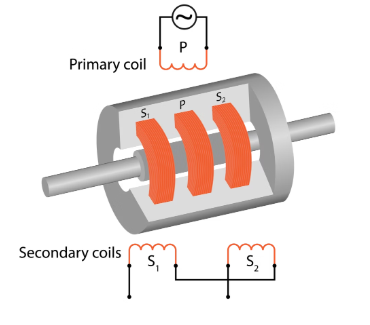
\includegraphics[width=0.3\linewidth]{img/LVDT}
	\caption{LVDT o Transormador diferencial}
	\label{fig:LVDT}
\end{figure}

\section{RESOLVER}
Un resolver\cite{ServoMotors_Resolver} es un sensor analógico de posición rotatoria, que a través de impulsos digitales puede regular la velocidad, la posición o el torque.

El resolver consiste en una parte estacionaria llamada estator y una parte giratoria llamada rotor, que es montada al eje del motor.

El bobinado primario del estator está conectado a una señal sinusoidal de alta frecuencia. Esta señal se transmite al bobinado del rotor, porque el bobinado primario del estator y el bobinado del rotor actúan juntos como un transformador. Además, podemos llamar el bobinado del rotor también como bobinado de referencia.
El campo magnético alternante pulsante del bobinado del rotor ahora induce una voltaje alterna en los bobinados de medición seno y coseno. Sus amplitudes, sin embargo, dependen de la posición angular del rotor.

Si el bobinado del rotor y el bobinado de medición están paralelos el uno al otro, el campo del rotor magnético pasa completamente por la bobina de medición y, por lo tanto, el voltaje inducido es máximo.

Sin embargo, si el bobinado del rotor y el bobinado de medición están en ángulos rectos el uno con el otro, no se producirá ningún voltaje.

Los resolvers se utilizan en los servo motores para diferentes sectores industriales (Robótica, automoción, packaging, food and beverage, etc…) en los que se utilizan máquinas accionadas eléctricamente para procesos definidos. Ya que son sistemas de realimentación robustos y fiables que controlan el régimen de un servomotor de forma precisa.